\thispagestyle{toancuabinone}
\pagestyle{toancuabi}
\everymath{\color{toancuabi}}
%\blfootnote{$^1$\color{toancuabi}...}
\graphicspath{{../toancuabi/pic2/}}
\begingroup
\AddToShipoutPicture*{\put(0,616){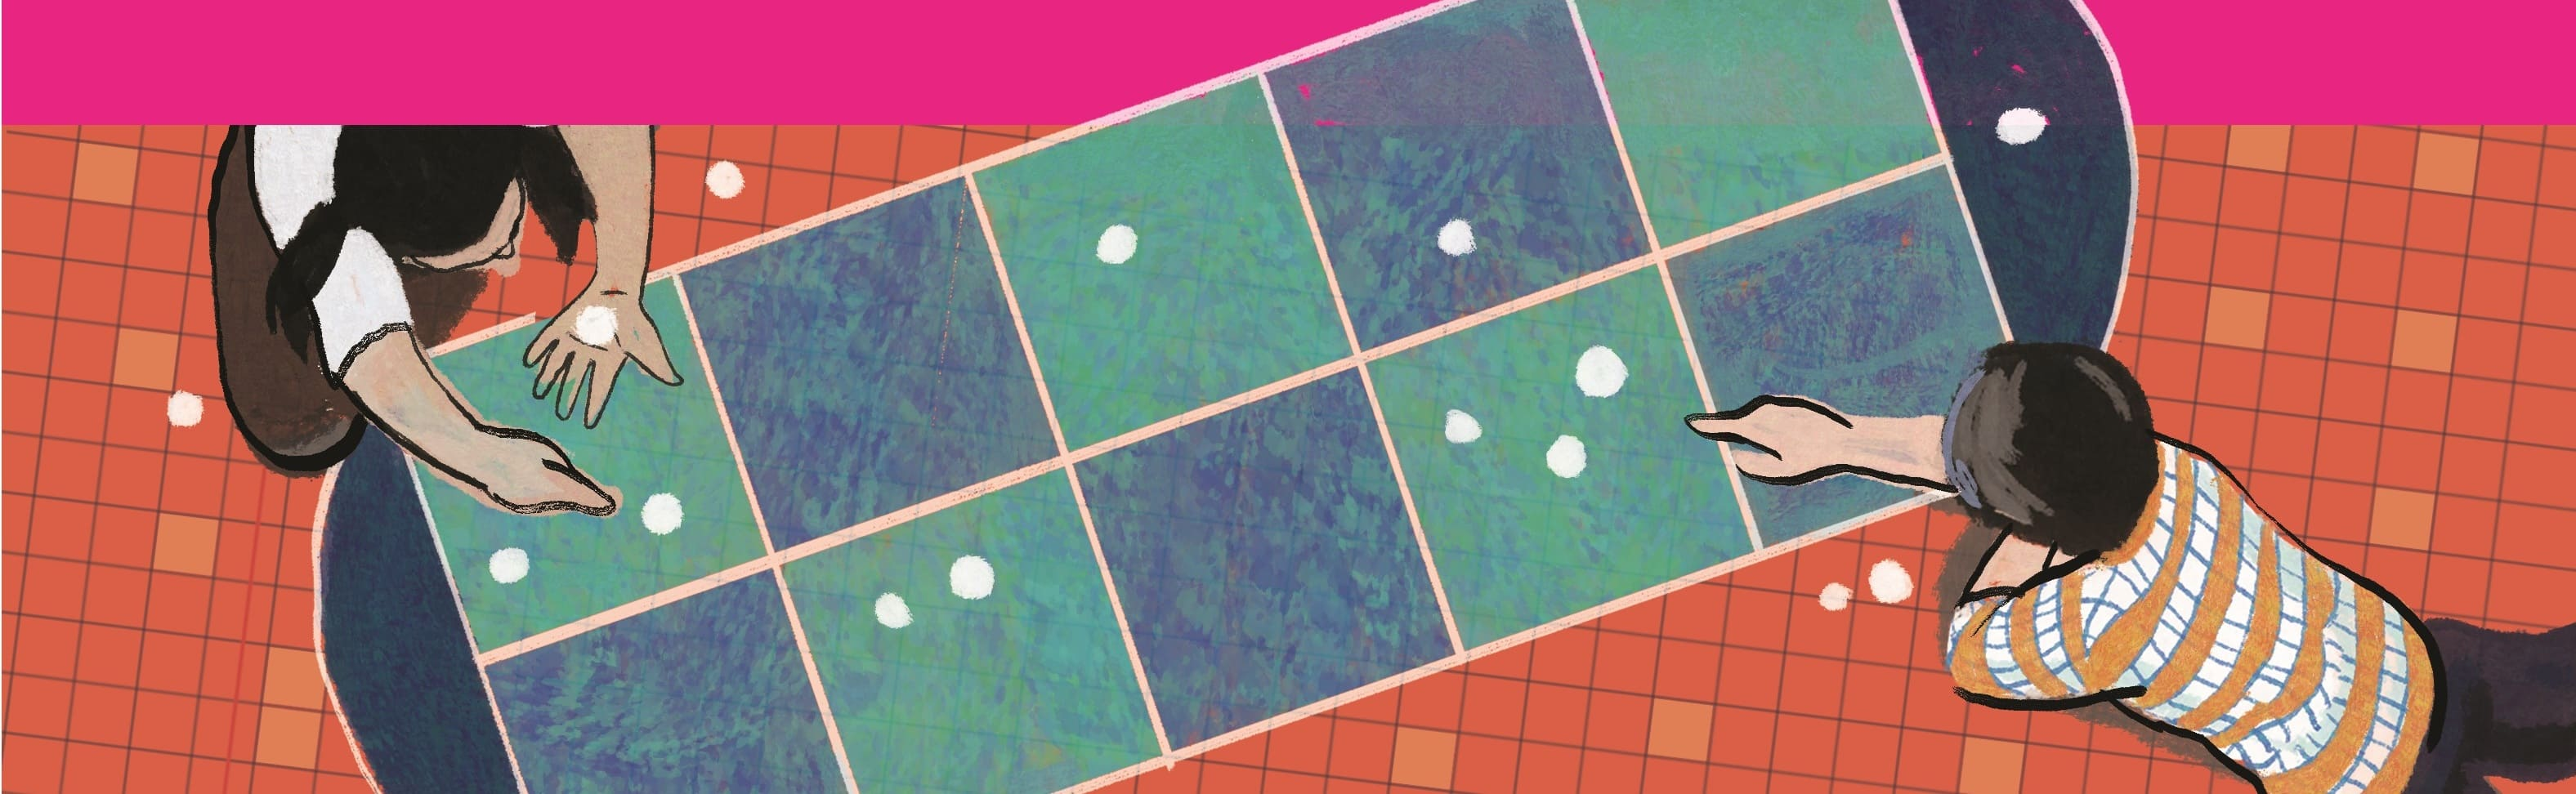
\includegraphics[width=19.3cm]{../bannertoancuabi}}}  
\AddToShipoutPicture*{\put(150,555){\includegraphics[scale=1]{../td.pdf}}} 
\centering
\endgroup
\vspace*{150pt}

\tikzset{
	pics/carc/.style args={#1:#2:#3}{
		code={
			\draw[pic actions] (#1:#3) arc(#1:#2:#3);
		}
	}
}
\begin{multicols}{2}
	Trong khi việc tính chu vi, diện tích của hình vuông, hình chữ nhật, hình tam giác,\ldots tương đối dễ hiểu, việc tính những số đo này cho hình tròn đã khiến các nhà toán học thời cổ đại băn khoăn trong thời gian khá dài. Dường như tính ``tròn trịa" của nó mang lại những thách thức không nhỏ!
	\vskip 0.1cm
	Chúng ta hãy bắt đầu với bài toán tính chu vi hình tròn. Lấy một tấm bìa, các em hãy dùng compa vẽ lên đó một đường tròn. Để tìm chu vi đường tròn, ta hãy đặt tấm bìa lên một chiếc thước kẻ, đánh dấu vị trí tiếp xúc rồi lăn nó cho đến khi điểm tiếp xúc quay được đủ $1$ vòng. Chu vi đường tròn là độ dài đoạn AB được minh họa trong hình vẽ sau.
	\begin{center}
		\resizebox{\columnwidth}{!}{\begin{tikzpicture}[scale=0.8,xshift=-2cm]
				% \draw[blue,  thick] (6.28,2.5)--(6.28,-7-1);
				%\draw[blue,  thick] (12.56,2.5)--(12.56,-7-1);
				\draw[step=.5cm,gray,very thin, dashed] (-0.4,-0.) grid (14.2,2.4); \draw (-.5,0) -- (14.5,0);
				\draw (0,0) -- (0,2.5);
				%\draw (0,-0.2) node[below] {O} tam bor
				\draw [very thick,draw=green!50!black]  (0,1) + (6.28,0) circle (1cm);
				\draw  [fill=red] (0,1) circle (0.1cm);
				\draw  [fill=red] (0,1) + (6.28,0) circle (0.1cm);
				%\draw (0,0)  + (6.28,0) node[below] {A}; tam bo
				\draw[very thick,draw=green!50!black] (0,1) circle (1 cm) pic[red, -latex]{carc=150:100:1.3cm};
				\draw  [fill=orange] (0,0) + (6.28,0) circle (0.09cm);
				\draw  [fill=orange] (0,0) circle (0.09cm);
				\draw (-0.2,0-1) rectangle (15.5,1-1);
				
				%% lower divisions
				\foreach \x in {0,1,...,15.5}{
					\draw (\x,0) -- (\x,-0.2)node[below,scale=0.4]{\x};
				}
				\foreach \x in {0.1,0.2,...,14.9}{
					\draw (\x,0) -- (\x,-0.075);
				}
				\foreach \x in {0.5,1,...,14.5}{
					\draw (\x,0) -- (\x,-0.15);
				}
				
				\draw[<->, orange, very thick] (0,0-1/2) -- (6.28,0-1/2);
				%        \draw[->, orange, very thick]   (4,0-1/2)--(6.28,-1/2);
				\node[orange] at (2.5+1/2,-0.8) {chu vi  đường tròn};
		\end{tikzpicture}}
	\end{center}
	Bây giờ, ta gấp đôi bán kính hình tròn, thực hiện lại việc đo chu vi của hình tròn mới và so sánh kết quả với trường hợp đầu nhé.
	\vskip 0.1cm
	Các em có nhận xét gì nào? Chu vi của hình tròn mới gấp đôi so với đường tròn cũ đúng không? Các em có thể thử thêm với hình tròn có đường kính gấp một số lần, chẳng hạn $3, 4,\ldots$ lần đường kính của đường tròn đã cho nữa nhé. Hẳn là các em đã đoán ra điều gì rồi phải không? Đúng thế, khi đường kính gấp lên $k$ lần chu vi sẽ gấp $k$ lần. Như vậy có nghĩa là tỷ số của chu vi đường tròn với đường kính  của nó là một số cố định không phụ thuộc kích thước hình tròn! 
	%	\begin{figure}[H]
		%		\vspace*{-5pt}
		%		\centering
		%		\captionsetup{labelformat= empty, justification=centering}
		%		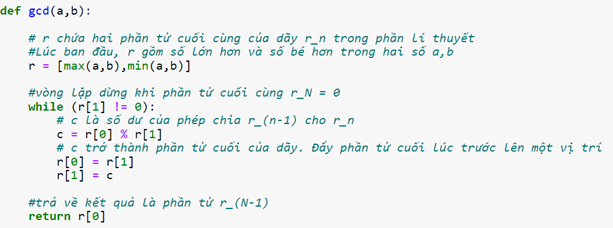
\includegraphics[width= 1\linewidth]{2}
		%		%		\caption{\small\textit{\color{toancuabi}Hình $1$.}}
		%		\vspace*{-10pt}
		%	\end{figure}
	\begin{center}
		\resizebox{\columnwidth}{!}{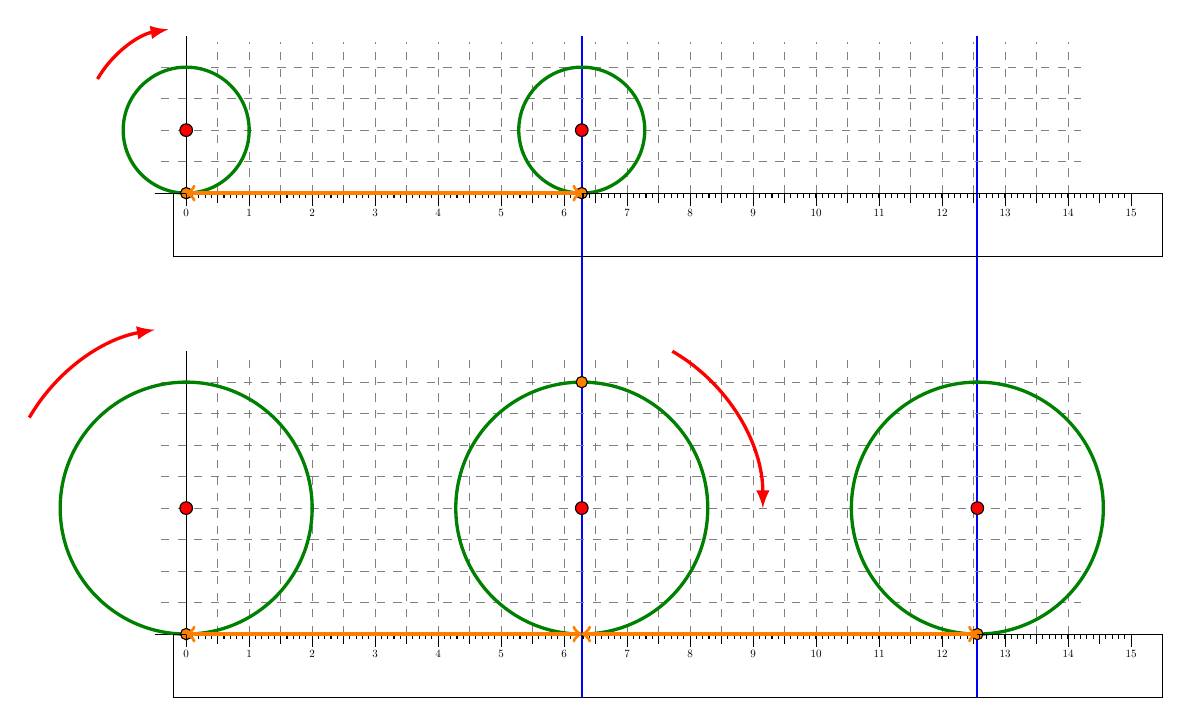
\begin{tikzpicture}[scale=0.8,xshift=-2cm]
				\draw[blue,  thick] (6.28,2.5)--(6.28,-7-1);
				\draw[blue,  thick] (12.56,2.5)--(12.56,-7-1);
				\draw[step=.5cm,gray,very thin, dashed] (-0.4,-0.) grid (14.2,2.4); \draw (-.5,0) -- (14.5,0);
				\draw (0,0) -- (0,2.5);
				%\draw (0,-0.2) node[below] {O} tam bor
				\draw [very thick,draw=green!50!black]  (0,1) + (6.28,0) circle (1cm);
				\draw  [fill=red] (0,1) circle (0.1cm);
				\draw  [fill=red] (0,1) + (6.28,0) circle (0.1cm);
				%\draw (0,0)  + (6.28,0) node[below] {A}; tam bo
				\draw[very thick,draw=green!50!black] (0,1) circle (1 cm) pic[red, -latex]{carc=150:100:1.3cm};
				\draw  [fill=orange] (0,0) + (6.28,0) circle (0.09cm);
				\draw  [fill=orange] (0,0) circle (0.09cm);
				\draw (-0.2,0-1) rectangle (15.5,1-1);
				
				%% lower divisions
				\foreach \x in {0,1,...,15.5}{
					\draw (\x,0) -- (\x,-0.2)node[below,scale=0.4]{\x};
				}
				\foreach \x in {0.1,0.2,...,14.9}{
					\draw (\x,0) -- (\x,-0.075);
				}
				\foreach \x in {0.5,1,...,14.5}{
					\draw (\x,0) -- (\x,-0.15);
				}
				
				%%%
				\draw[step=.5cm,gray,very thin, dashed] (-0.4,-0-7) grid (14.2,4.4-7); \draw (-.5,-7) -- (14.5,0-7);
				\draw (0,0-7) -- (0,4.5-7);
				%\draw (0,-0.2-7) node[below] {O}; tam bo
				\draw  [fill=red] (0,2-7) circle (0.1cm);
				\draw  [fill=red] (0,2-7) + (6.28,0) circle (0.1cm);
				\draw  [fill=red] (0,2-7) + (12.56,0) circle (0.1cm);
				%\draw (0,0-7)  + (6.28,0-7) node[below] {A};
				\draw[very thick,draw=green!50!black] (0,2-7) circle (2 cm) pic[red, -latex]{carc=150:100:2.3cm};
				\draw [very thick,draw=green!50!black]  (0,2-7) + (6.28,0) circle (2cm) pic[red, -latex]{carc=60:0:2.3cm};;
				\draw [very thick,draw=green!50!black]  (0,2-7) + (12.56,0) circle (2cm);
				\draw  [fill=orange] (0,0-7) + (12.56,0) circle (0.09cm);
				\draw  [fill=orange] (0,0-7) circle (0.09cm);
				\draw  [fill=orange] (0,0-7) + (6.28,4) circle (0.09cm);
				%%%%%
				\draw (-0.2,0-1-7) rectangle (15.5,1-1-7);
				%% lower divisions
				\foreach \x in {0,1,...,15.5}{
					\draw (\x,0-7) -- (\x,-0.2-7)node[below,scale=0.4]{\x};
				}
				\foreach \x in {0.1,0.2,...,14.9}{
					\draw (\x,0-7) -- (\x,-0.075-7);
				}
				\foreach \x in {0.5,1,...,14.5}{
					\draw (\x,0-7) -- (\x,-0.15-7);
				}
				
				
				\draw[<->, orange, very thick] (0,0) -- (6.28,0);
				\draw[<->, orange, very thick] (0,0-7) -- (6.28,0-7);
				\draw[<->, orange, very thick] (12.56,-7) -- (6.28,0-7);
		\end{tikzpicture}}
	\end{center}
	Ngược lại dòng thời gian, khoảng $2000$ năm trước công nguyên, người Babylon, Ai Cập và Trung Quốc một cách độc lập đã cùng đưa ra được nhận xét này. Sau này vào đầu thế kỉ $18$ một nhà toán học tên là William Jones dùng $\pi$ để kí hiệu tỷ số trên, xuất phát từ $\pi$ là chữ cái đầu tiên trong chữ ``\textit{περιϕέρεια}" của tiếng Hy Lạp và có nghĩa là ``chu vi đường tròn".
	\vskip 0.1cm
	Từ đây ta có công thức tính chu vi đường tròn có bán kính $r$ (sgk: viết là chu vi hình tròn)
	\begin{align*}
		C=\pi\times2\times r.
	\end{align*}
	Dường như, trong một thời gian dài không có thêm cải tiến nào cho việc tính xấp xỉ cũng như hiểu thêm về $\pi$. Sự kiện đột phá là phương pháp tính xấp xỉ của Archimedes, nhà bác học vĩ đại của Hy Lạp sống vào khoảng những năm $250$ TCN. Trong bài viết này ta sẽ tìm hiểu xem Archimedes đã tính xấp xỉ số $\pi$ và tính diện tích hình tròn như thế nào nhé.
	\begin{figure}[H]
		\vspace*{-5pt}
		\centering
		\captionsetup{labelformat= empty, justification=centering}
		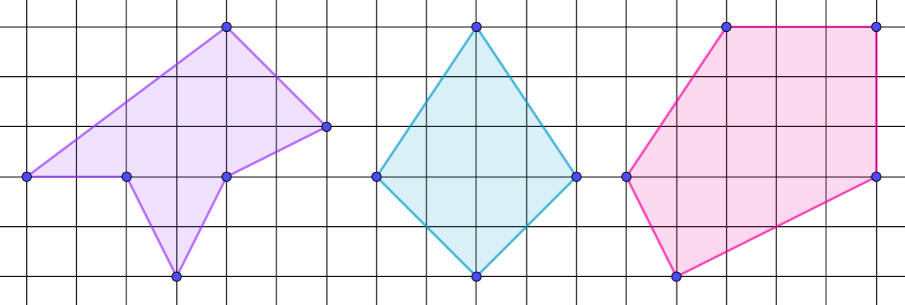
\includegraphics[width= 0.5\linewidth]{3}
		%		\caption{\small\textit{\color{toancuabi}Hình $1$.}}
		\vspace*{-10pt}
	\end{figure}
	Số Pi gắn bó mật thiết với bài toán tính chu vi và diện tích hình tròn. Năm bài toán trong số những bài toán viết trên cuộn giấy Rhind  có liên quan tới tính diện tích hình tròn, trong đó người ta xấp xỉ $\pi$ bằng một số gần bằng $3$ khi thực hiện việc tính toán. 
	\begin{figure}[H]
		\vspace*{-5pt}
		\centering
		\captionsetup{labelformat= empty, justification=centering}
		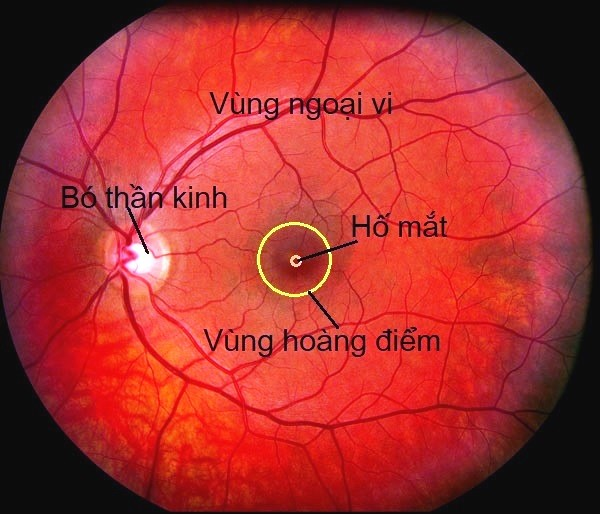
\includegraphics[width= 1\linewidth]{4}
		\caption{\small\textit{\color{toancuabi}Cuộn giấy Rhind: một cuộn giấy có nguồn gốc từ Ai Cập cổ, trên đó viết một số bài toán và cách giải chúng. Tên cuộn giấy được đặt theo tên nhà sưu tầm đồ cổ, Alexander Henry Rhind, người đã mua nó ở Ai Cập năm $1858$.}}
		\vspace*{-10pt}
	\end{figure}
	\textbf{\color{toancuabi}Xấp xỉ số} $\pmb{\pi}$ 
	\vskip 0.1cm
	Ý tưởng xấp xỉ của Archimedes xuất phát từ quan sát sau đây: Vẽ hai  đa giác $n$ đỉnh, một đa giác nằm trong đường tròn, một đa giác chứa đường tròn bên trong. Nếu ta chọn đường tròn có đường kính bằng $1$ thì chu vi đường tròn chính là số $\pi$.  Gọi chu vi các đa giác và đường tròn lần lượt là $c_n$, $C_n $và $C$, khi đó
	\begin{align*}
		{\color{red}c_n} < {\color{green}C} < {\color{blue}C_n}.
	\end{align*}
	Chu vi đa giác màu đỏ < chu vi đường tròn màu xanh lá < chu vi đa giác màu xanh dương
	\begin{figure}[H]
		\vspace*{-5pt}
		\centering
		\captionsetup{labelformat= empty, justification=centering}
		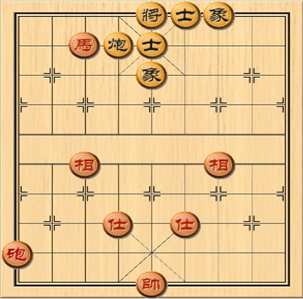
\includegraphics[width= 1\linewidth]{5}
		\caption{\small\textit{\color{toancuabi}\hfill$n=3$\hfill\quad $n= 6$ \quad\quad\, $n= 12$.\quad}}
		\vspace*{-10pt}
	\end{figure}
	Nhận thấy khi tăng $n$ thì lên $c_n,C_n$ sẽ ngày càng gần $C$ tức ngày càng gần $\pi$.  Như vậy, việc tính được diện tích của các đa giác ta sẽ tính được gần đúng $\pi$. Hơn nữa, các đa giác càng nhiều đỉnh thì việc xấp xỉ càng chính xác. Archimedes lựa chọn các đa giác đều để thuận lợi hơn cho việc tính độ dài các cạnh của nó: Xuất phát từ tam giác đều rồi lục giác đều,\ldots\, và cuối cùng bằng những kiến thức hình học của mình, ông đã sử dụng đa giác đều có $96$ đỉnh và tìm được $\pi$ nằm giữa $3+ 10/70$ và $3+10/71$ ($3{.}1408$ và $3{.}1429$). Thật tuyệt!
	\vskip 0.1cm
	Với những kiến thức sẽ được học ở các cấp học sau và với sự trợ giúp của máy tính, các em có thể tính được số Pi nằm giữa những cặp giá trị trong bảng sau bằng cách dùng những đa giác đều tương tự như Archimedes đã dùng.
	\begin{table}[H]
		\vspace*{-5pt}
		\setlength{\tabcolsep}{7pt}
		\renewcommand{\arraystretch}{1.3}
		\begin{tabular}{|c|c|c|}
			\hline
			Số cạnh đa giác $(n)$ & $\color{red}c_n$ & $\color{blue}C_n$\\
			\hline
			$3$ &	$\color{red}2,5981$&	$\color{blue}5,1962$\\
			\hline
			$6$&	$\color{red}3$&	$\color{blue}3,4641$\\
			\hline
			$12$&	$\color{red}3,1058$&	$\color{blue}3,2154$\\
			\hline
			$24$& $\color{red}3,1326$&	$\color{blue}3,1596$\\
			\hline
			$48$&	$\color{red}3,1394$&	$\color{blue}3,1461$\\
			\hline
			$96$&	$\color{red}3,1410$&	$\color{blue}3,1427$\\
			\hline
		\end{tabular}
		\vspace*{-10pt}
	\end{table}
	Đến đây các em đã hiểu tại sao người ta lấy $3{.}14$ làm số xấp xỉ $\pi$ rồi phải không ? Từ đây, ta cũng có công thức tính chu vi đường tròn như sau
	\begin{align*}
		C=3{.}14\times2\times r.
	\end{align*}
	Sau Archimedes, nhiều nhà toán học tiếp tục tìm cách xấp xỉ $\pi$  bằng nhiều phương pháp khác nhau. Ngày nay với sự trợ giúp của máy tính chúng ta có thể xấp xỉ $\pi$ với độ chính xác rất cao.
	\vskip 0.1cm
	\textbf{\color{toancuabi}Diện tích hình tròn}
	\vskip 0.1cm
	Với ý tưởng tương tự, Archimedes xem xét cách tính diện tích của hình tròn có bán kính $r$. Ông chia nó ra thành nhiều mảnh bằng nhau. Diện tích của  hình tròn là tổng diện tích những mảnh nhỏ đó.
	\begin{figure}[H]
		\vspace*{-5pt}
		\centering
		\captionsetup{labelformat= empty, justification=centering}
		\includegraphics[width= 0.65\linewidth]{p1}
		%		\caption{\small\textit{\color{toancuabi}\hfill$n=3$\hfill $n= 6$ \hfill $n= 12$.\hfill}}
		\vspace*{-10pt}
	\end{figure}
	Nếu ta chia hình tròn thành $4$ mảnh và sau đó ta ghép chúng lại thì được hình sau. Ta có thể thấy ngay đường viền màu đỏ là nửa chu vi, đường màu xanh bằng bán kính $r$.
	\begin{figure}[H]
		\vspace*{-5pt}
		\centering
		\captionsetup{labelformat= empty, justification=centering}
		\includegraphics[width= 1\linewidth]{p2}
		%		\caption{\small\textit{\color{toancuabi}\hfill$n=3$\hfill $n= 6$ \hfill $n= 12$.\hfill}}
		\vspace*{-10pt}
	\end{figure}
	Trông nó thật lạ các em nhỉ! Ta thử tiếp bằng cách chia hình tròn thành $8$ phần (bằng cách chia đôi những mảnh nhỏ ở trên) và sau đó ghép lại.
	\begin{figure}[H]
		\vspace*{5pt}
		\centering
		\captionsetup{labelformat= empty, justification=centering}
		\includegraphics[width= 1\linewidth]{p3}
		%		\caption{\small\textit{\color{toancuabi}\hfill$n=3$\hfill $n= 6$ \hfill $n= 12$.\hfill}}
		\vspace*{-10pt}
	\end{figure}
	Ta cũng quan sát thấy điều tương tự: đường màu đỏ là nửa chu vi và màu xanh là bán kính. Trông nó khá giống một hình bình hành phải không? Ta dùng kéo cắt hai đầu và ghép lại một lần nữa để được hình sau.
	\begin{figure}[H]
		\vspace*{-5pt}
		\centering
		\captionsetup{labelformat= empty, justification=centering}
		\includegraphics[width= 1\linewidth]{p4}
		%		\caption{\small\textit{\color{toancuabi}\hfill$n=3$\hfill $n= 6$ \hfill $n= 12$.\hfill}}
		\vspace*{-10pt}
	\end{figure}
	Các em thấy sao? Hình vẽ ta thu được trông khá giống một hình chữ nhật nhỉ? Tương tự ta vẫn có đường màu đỏ có độ dài nửa chu vi đường tròn $C/2$, đường màu xanh có độ dài bằng bán kính $r$ như trên.
	\vskip 0.1cm
	Ta tiếp tục cắt đôi mỗi mảnh và ghép lại theo cách tương tự
	\begin{figure}[H]
		\vspace*{-5pt}
		\centering
		\captionsetup{labelformat= empty, justification=centering}
		\includegraphics[width= 1\linewidth]{p5}
		%		\caption{\small\textit{\color{toancuabi}\hfill$n=3$\hfill $n= 6$ \hfill $n= 12$.\hfill}}
		\vspace*{-10pt}
	\end{figure}
	Các em có nhận xét gì về độ nhấp nhô của đường màu đỏ? Dường như càng ngày nó càng ``thẳng" hơn. Tưởng tượng xem nếu ta cứ tiếp tục như thế thật lâu ta sẽ thu được hình càng ngày càng gần với một hình chữ nhật có một cạnh là $C/2$, cạnh còn lại là $r$. Quan sát thấy điều đó Archimede kết luận rằng diện tích hình tròn chính là diện tích hình chữ nhật ``lý tưởng" nói trên. Ý tưởng chia thật  nhỏ và ghép lại này thật là hay!
	\begin{figure}[H]
		\vspace*{-5pt}
		\centering
		\captionsetup{labelformat= empty, justification=centering}
		\includegraphics[width= 1\linewidth]{p6}
		%		\caption{\small\textit{\color{toancuabi}\hfill$n=3$\hfill $n= 6$ \hfill $n= 12$.\hfill}}
		\vspace*{-10pt}
	\end{figure}
	Vậy ta thu được công thức tính diện tích hình tròn có bán kính $r$ là
	\begin{align*}
		S &= \frac{C}{2} \times r = \pi \times r \times r \\
		&\approx 3{.14} \times r \times r.
	\end{align*}
	Ý tưởng của Archimedes được sử dụng và phát triển trong nhiều lĩnh vực khác của toán học mà đáng chú ý nhất có lẽ là trong giải tích, một lĩnh vực toán học có rất nhiều ứng dụng trong thực tiễn.
	\vskip 0.1cm
	\textbf{\color{toancuabi}Tài liệu tham khảo}
	\vskip 0.1cm
	[$1$] 1, R. L. Cooke, ``The history of mathematics", John Wiley \& Sons, Inc, $2013$.
	\vskip 0.1cm
	[$2$] S. Strogatz, ``Infinite Powers How Calculus Reveals the Secrets of the Universe", Houghton Mifflin Harcourt Publishing Company, $2019$. 
	\vskip 0.1cm
	[$3$] Infinite Powers How Calculus Reveals the Secrets of the Universe by Steven H. Strogatz (z-lib.org).pdf
	\vskip 0.1cm
	[$4$] How Archimedes showed that $\pi$ is approximately equal to $22/7$. DaminiD.B. and AbhishekDhar 
	\vskip 0.1cm
	[$5$] \url{http://www.ams.org/publicoutreach/feature-column/fc-2012-02}
	\vskip 0.1cm
	[$6$] From $0$ to Infinity in $26$ Centuries: The Extraordinary Story of Maths
\end{multicols}
\vspace*{-10pt}
\rule{1\linewidth}{0.1pt}
\begingroup
\AddToShipoutPicture*{\put(72,430){
\includegraphics[scale=1]{../tieude.pdf}}} 
\centering
\endgroup
\vspace*{38pt}

\begin{multicols}{2}
	Tám người với nghề nghiệp khác nhau vừa bị trộm sạch tiền bởi tên trùm lừa đảo với biệt danh Ông Cạ. Các nạn nhân này quyết định gặp  nhau để chia buồn an ủi và bàn cách truy tìm Ông Cạ gian manh. Họ mời cả bên sở cảnh sát và văn phòng thám tử tới tham dự buổi họp đặc biệt đó. Khi Xuân Phong tới nơi, thám tử thấy tám người này ngồi xung quanh một chiếc bàn (xem sơ đồ dưới đây). Từ các thông tin sau, các em có thể tìm ra vị trí cụ thể của mỗi người và nghề nghiệp của họ được hay không?
	\begin{figure}[H]
		\vspace*{-5pt}
		\centering
		\begin{tikzpicture}[scale=0.65]
			\draw[color=cackithi] (0,0) rectangle (9,3);
			\draw (0.5,-0.5) node {$(8)$};
			\draw (-0.5,1.5) node {$(1)$};
			\draw (0.5,3.5) node {$(2)$};
			\draw (4.5,-0.5) node {$(7)$};
			\draw (4.5,3.5) node {$(3)$};
			\draw (8.5,-0.5) node {$(6)$};
			\draw (9.5,1.5) node {$(5)$};
			\draw (8.5,3.5) node {$(4)$};
		\end{tikzpicture}
		\vspace*{-20pt}
	\end{figure}
	$1.$	Bác sỹ thú y và Nha sỹ ngồi đối diện nhau.
	\vskip 0.05cm
	$2.$	Chủ tọa buổi họp ngồi ở vị trí $(1)$ với người tên là An ngồi bên trái.
	\vskip 0.05cm
	$3.$	Người tên là Vũ ngồi ở vị trí đánh số chẵn với ông Nhân viên ngân hàng ngồi bên trái~mình.
	\vskip 0.05cm
	$4.$ Bác sỹ đa khoa có người làm nghề Cố vấn pháp luật ngồi bên tay phải.
	\begin{figure}[H]
		\vspace*{-5pt}
		\centering
		\captionsetup{labelformat= empty, justification=centering}
		\includegraphics[width= 1\linewidth]{xp}
		\vspace*{-10pt}
	\end{figure}
	$5.$	Ông Công, chứ không phải ông Bình, ngồi ở vị trí $(3)$, đối diện trực tiếp với người là Kỹ sư xây dựng
	\vskip 0.05cm
	$6.$	Người thợ làm bánh ngồi ở vị trí số $(5)$  với ông Trung ngồi bên trái và ông Đức ngồi bên phải.
	\vskip 0.05cm
	$7.$	Người tên là Sinh ngồi bên trái Bác sỹ thú~y.
	\vskip 0.05cm
	$8.$	Người tên là Bửu, ngồi đối diện với ông Công, có Bác sỹ phẫu thuật ngồi bên tay trái mình.
\end{multicols}
\newpage
\begingroup
\AddToShipoutPicture*{\put(110,670){
\includegraphics[scale=1]{../tieude11.pdf}}} 
\centering
\endgroup
\vspace*{45pt}

\begin{multicols}{2}
	$\pmb{1.}$	Một số các bạn học sinh lớp $7$ đứng xếp  thành hàng ngang. Trước mặt mỗi bạn lại có một học sinh lớp $6$ thấp hơn về chiều cao đứng đối diện. Em hãy chứng tỏ rằng nếu $2$ hàng ngang của các học sinh lớp $7$ và lớp $6$ được xếp lại tăng dần theo chiều cao ở mỗi hàng, thì ở hai hàng mới, mỗi học sinh lớp $7$ lại vẫn như cũ, sẽ đứng đối diện với một học sinh lớp $6$ thấp hơn mình.
	\begin{figure}[H]
		\vspace*{-5pt}
		\centering
		\captionsetup{labelformat= empty, justification=centering}
		\includegraphics[width= 1\linewidth]{b1}
		\vspace*{-15pt}
	\end{figure}
	$\pmb{2.}$	Trên một bàn cờ vua người ta đặt một số quân cờ mà ở  mỗi một hàng ngang và mỗi hàng dọc của bàn cờ đều có một số lẻ các quân cờ. Em hãy chứng tỏ rằng có một số chẵn các quân cờ đứng ở các ô màu đen của bàn cờ đó.
	\begin{figure}[H]
		\vspace*{-5pt}
		\centering
		\captionsetup{labelformat= empty, justification=centering}
		\includegraphics[width= 1\linewidth]{b2}
		\vspace*{-15pt}
	\end{figure}
	$\pmb{3.}$	Trên bảng có ghi một số các số nguyên mà hai số bất kì trong đó là khác nhau.  Hơn nữa tổng của hai số bất kỳ trong chúng cũng được ghi trên đó. Hỏi có bao nhiêu số được viết ra trên bảng?
	\vskip 0.1cm
	$\pmb{4.}$	Trong một buổi cắm trại có $9$ học sinh nam và $10$ học sinh nữ tham gia. Trước đó, mỗi học sinh nam đều đã quen với cùng một số lượng các học sinh nữ tham gia buổi cắm trại đó, còn tất cả các học sinh nữ đều quen số lượng học sinh nam hoàn toàn khác nhau (không có hai em nữ nào có số lượng bạn nam quen biết giống nhau). Hỏi điều này có thể xảy ra hay không?
	\begin{figure}[H]
		\vspace*{-5pt}
		\centering
		\captionsetup{labelformat= empty, justification=centering}
		\includegraphics[width= 1\linewidth]{b4}
		\vspace*{-15pt}
	\end{figure}
	$\pmb{5.}$	Trong một giải thi đấu bóng chuyền, mỗi đội sẽ lần lượt thi đấu với các đội còn lại hai lần. Cuối cùng người ta thấy rằng $80\%$ các đội có ít nhất một trận thắng. Hỏi có tất cả bao nhiêu đội đã tham gia trong giải đấu đó biết rằng các trận đấu bóng chuyền không có tỷ số hoà?
	\begin{figure}[H]
		\vspace*{-5pt}
		\centering
		\captionsetup{labelformat= empty, justification=centering}
		\includegraphics[width= 1\linewidth]{b5}
		\vspace*{-15pt}
	\end{figure}
	$\pmb{6.}$	Bốn chú lùn cùng đi chẻ củi để chuẩn bị cho một mùa đông có nàng Bạch Tuyết tới ở cùng, họ chẻ mất  $3$ tiếng đồng hồ. Nếu như chú lùn thứ nhất làm nhanh gấp đôi, còn chú thứ hai làm chậm một nửa, thì $4$ chú cũng sẽ hoàn thành trong từng đó thời gian. Còn nếu như, ngược lại, chú thứ nhất làm chậm một nửa, còn chú thứ hai làm nhanh gấp đôi, thì họ sẽ xoay sở  đống củi chỉ trong $2$ tiếng.
	\vskip 0.1cm
	Hỏi $3$ chú lùn đầu tiên sẽ chẻ hết đống củi trong bao nhiêu lâu mà không cần sự trợ giúp của chú thứ tư?
	\begin{figure}[H]
		%		\vspace*{-5pt}
		\centering
		\captionsetup{labelformat= empty, justification=centering}
		\includegraphics[width= 1\linewidth]{b6}
		\vspace*{-10pt}
	\end{figure}
\end{multicols}
\vspace*{-10pt}
\rule{1\linewidth}{0.1pt}
\begingroup
\AddToShipoutPicture*{\put(112,450){
\includegraphics[scale=1]{../tieude2.pdf}}} 
\centering
\endgroup
\vspace*{80pt}

\begin{multicols}{2}
	$\pmb{1.}$ Sắp đến thời gian các chú tí hon phải trở về thành phố Hoa, thi sĩ Hoa Giấy và thi sĩ Hoa Lan đều làm những bài thơ tặng các bạn của mình. Vì nóng lòng muốn đọc ngay bài thơ mình vừa sáng tác, sáng sớm hôm sau, hai thi sĩ cùng đi sớm nhất có thể (thế nên cùng thời điểm) để đến nhà nhau. Vì mải ngâm thơ dọc đường nên hai bạn không nhìn thấy nhau tại lúc gặp nhau giữa đường. Sau thời điểm gặp, Hoa Lan đến nhà Hoa Giấy sau đó $4$ phút, còn Hoa Giấy đến nhà Hoa Lan sau đó $1$ phút. Các bạn hãy tính xem mỗi thi sĩ đã đi đến nhà nhau mất bao nhiêu phút nhé.
	\begin{figure}[H]
		\centering
		\vspace*{-5pt}
		\captionsetup{labelformat= empty, justification=centering}
		\includegraphics[height=0.5\linewidth]{ToanBi_12_Hinh1_HoaGiay}\quad\quad
		\includegraphics[height=0.5\linewidth]{ToanBi_12_Hinh2_HoaDai}
		\vspace*{-10pt}
	\end{figure} 
	\textit{Lời giải.} Gọi $a$ là số thời gian tính theo phút từ lúc hai thi sĩ khởi hành tới lúc gặp nhau. Vận tốc của Kèn Đồng là $g$, vận tốc của Hoa Dại là $d$, khi đó ta có quãng đường từ nhà Hoa Dại tới điểm gặp là $da$, quãng đường từ nhà Kèn Đồng tới điểm gặp là $ga$. Sau khi gặp, Kèn Đồng đi tiếp $1g$ còn Hoa Dại đi tiếp $4d$.
	\begin{figure}[H]
		\centering
		\vspace*{-5pt}
		\captionsetup{labelformat= empty, justification=centering}
		\begin{tikzpicture}[color=toancuabi,scale=0.85]
			\draw (0,0) -- (6,0);
			\draw (0,2) -- (6,2);
			\draw[align=left] (0,2) node [left] {Kèn\\Đồng};
			\draw[align=left] (6,0) node [right] {Hoa\\Dại};
			\node[circle, fill=cackithi,inner sep=0pt, minimum size=5pt] (b) at (4,2) {};
			\node[circle, fill=cackithi,inner sep=0pt, minimum size=5pt] (b) at (4,0) {};
			\draw (2,0) node[above] {$ag$};
			\draw (2,2) node[above] {$4d$};
			\draw (5,0) node[above] {$ad$};
			\draw (5,2) node[above] {$1g$};
		\end{tikzpicture}
		\vspace*{-15pt}
	\end{figure} 
	So sánh quãng đường từ lúc khởi hành đến lúc gặp theo hai cách, ta có $1g = da$ và $4d=ga$.
	\vskip 0.1cm
	Nhân hai vế của hai đẳng thức trên với nhau ta có $4dg= a\cdot a\cdot gd$. Giản ước cho $gd$ ta có  $a\cdot a=4$. Số a duy nhất thỏa mãn là $a=2$. Vậy Hoa Dại đi mất $2+4 = 6$ phút, còn Kèn Đồng đi mất $2+1 = 3$ phút.
	\vskip 0.1cm
	$\pmb{2.}$ Để làm kỷ niệm, Mắt Xanh và một số cô tí hon trong thành phố Xanh đã may túi tặng các chú tí hon. Mỗi cô trong nhóm đã may được một số lượng túi như nhau và cùng nhau mang túi đến tập hợp ở nhà Bạch Tuyết. 
	Trên đường đi, các cô gặp một nhóm các chú tí hon và thật trùng hợp số chú tí hon trong nhóm đúng bằng số các cô tí hon, mỗi cô đã tặng mỗi chú tí hon một chiếc túi mà mình may được. Sau khi tặng túi, mỗi cô tí hon vẫn còn hơn $1$ chiếc và tập hợp tất cả lại được $33$ chiếc mang đến nhà Bạch Tuyết. Các bạn có tính được mỗi cô tí hon đã may bao nhiêu chiếc túi không?
	\begin{figure}[H]
		\centering
		\vspace*{-5pt}
		\captionsetup{labelformat= empty, justification=centering}
		\includegraphics[width=1\linewidth]{ToanBi_12_Hinh3_TangTui}
		\vspace*{-15pt}
	\end{figure}
	\textit{Lời giải.} Gọi số cô tí hon là $a$, số túi mỗi cô đã may được là $b$. Khi đó, tổng số túi các cô tí hon đã làm được là $ab$. Mỗi cô tí hon đã tặng $a$ túi cho mỗi chú tí hon, vì vậy có tất cả $a\times a$ số túi được tặng đi. Vì thế, cuối cùng các cô đã mang đến $ab - a\times a$ túi đến nhà Bạch Tuyết.
	\vskip 0.1cm
	Ta có $ab - a\times a =33$, hay là $a(b-a) = 33$. Do đó, $a$ là ước số của $33$. Theo đề bài, do $b - a > 1$ và $a>1$ nên $a$ phải khác $1$ và $33$, vì thế $a=3$ hoặc $a= 11$.
	\begin{table}[H]
		\centering
		\setlength{\tabcolsep}{10pt}
		\renewcommand{\arraystretch}{1.3}
		\begin{tabular}{|c|c|c|}
			\hline
			$a$&	$3$&	$11$\\
			\hline
			$b - a$&	$11$&	$3$\\
			\hline
			$b$&	$14$&	$14$\\
			\hline
		\end{tabular}
	\end{table}
	Trong cả hai trường hợp, chúng ta thấy số túi các cô tí hon may được đều bằng $14$.
	\vskip 0.1cm
	$\pmb{3.}$ Một buổi vũ hội đã được tổ chức trước ngày các chú tí hon trở về. Cuối buổi, các cô chú tí hon xếp thành một vòng tròn để nghe hai thi sĩ Hoa Giấy và Hoa Lan đọc thơ. Mít Đặc và Tròn Xoay mải chạy loanh quanh nên không kịp tham gia vào vòng tròn này. 
	\vskip 0.1cm
	Tròn Xoay nói: ``Tớ chưa từng thấy nhiều người trong một vòng tròn như thế. Chúng ta đếm thử xem có bao nhiêu người nhé." Mít Đặc và Tròn Xoay cùng đi theo một chiều để đếm số người trong vòng tròn nhưng bắt đầu từ những người khác nhau. Người thứ $20$ theo cách đếm của Mít Đặc lại là người thứ $7$ theo cách đếm của Tròn Xoay, còn người thứ $7$ theo cách của đếm của Mít Đặc lại là người thứ $94$ theo cách của Tròn Xoay. Thế thì vòng tròn này có bao nhiêu cô chú tí hon nhỉ? Các bạn có tính được không?
	\begin{figure}[H]
		\centering
		\vspace*{-5pt}
		\captionsetup{labelformat= empty, justification=centering}
		\includegraphics[width=0.7\linewidth]{ToanBi_12_Hinh4_VuHoi}
		\vspace*{-15pt}
	\end{figure}
	\textit{Lời giải.} Theo thông tin từ bài, người đầu tiên (người số $1$) của Tròn Xoay phải là người số $14$ của Mít Đặc. Vì thế người ở vị trí cuối cùng của Tròn Xoay sẽ là người số $13$ theo cách đếm của Mít Đặc. Từ đó suy ra hiệu số của các số thứ tự của người số $94$ và người cuối cùng theo cách đếm của Tròn Xoay cũng chính là hiệu số giữa số thứ tự của người số $7$ và người số $13$ theo cách đếm của Mít Đặc. Vì thế người cuối cùng là người số: $94+ 13-7=100$ theo cách đếm của Tròn Xoay.
	\begin{figure}[H]
		\centering
		\vspace*{-5pt}
		\captionsetup{labelformat= empty, justification=centering}
		\includegraphics[width=0.8\linewidth]{gb3}
		\vspace*{-10pt}
	\end{figure}
	Vậy vòng tròn trong buổi vũ hội có $100$ cô chú tí hon.
	\vskip 0.1cm
	$\pmb{4.}$ Khi chia tay với các cô tí hon, Mít Đặc hứa là sẽ viết thư cho Mắt Xanh, thế nên từ khi trở về thành phố Hoa, cậu chịu khó luyện viết lắm, dạo này cậu còn học thêm cả toán nữa. Trong bức thư trước, Mắt Xanh hỏi bao giờ thì các chú làm xong khinh khí cầu để quay lại thăm thành phố Xanh.
	\begin{figure}[H]
		\centering
		\vspace*{-5pt}
		\captionsetup{labelformat= empty, justification=centering}
		\includegraphics[width=0.23\textwidth]{ToanBi_12_Hinh5_MitDac}
		\vspace*{-10pt}
	\end{figure}
	Trong bức thư lần này gửi cho Mắt Xanh, Mít Đặc được dịp thể hiện luôn, cậu viết: ``Chúng tớ đang làm khinh khí cầu rồi. Biết Tuốt đã dự tính một số ngày. Nếu mỗi người bọn tớ làm $6$ ngày công thì sẽ thừa ra $20$ ngày, còn nếu mỗi người chỉ làm $4$ ngày công thì vừa đủ so với dự tính. Cậu thử tính xem Biết Tuốt dự kiến bao nhiêu ngày". Các bạn hãy tính cùng Mắt Xanh nhé.
	\vskip 0.1cm
	\textit{Lời giải.} Theo hình vẽ bên, ta thấy số ngày dự tính làm kinh khí cầu bằng số chú tí hon tham gia vào làm nhân với mỗi ngày làm của mỗi chú.
	\vskip 0.1cm
	Số chú tí hon tham gia vào làm kinh khí cầu là: $20 : 2 = 10$ (người)
	\vskip 0.1cm
	Số ngày cần thiết để làm kinh khí cầu là: $10 \times 4 = 40$ (ngày)
	\begin{figure}[H]
		\centering
		\vspace*{-5pt}
		\captionsetup{labelformat= empty, justification=centering}
		\includegraphics[width=1\linewidth]{gb4}
		\vspace*{-10pt}
	\end{figure}
\end{multicols}

%\thispagestyle{toancuabinone}
%\blfootnote{\color{toancuabi}$^1$Archimedes Academy.}
\begingroup
%\AddToShipoutPicture*{\put(-2,733){\includegraphics[width=17.2cm]{../math8.pdf}}} 
\AddToShipoutPicture*{\put(90,445){
\includegraphics[scale=1]{../tieude3.pdf}}} 
\centering
\endgroup

\vspace*{55pt}

\begin{multicols}{2}
	In this series of articles, we discuss mathematical reasoning by a number of examples. Let's start with a few classic examples.
	These problems are simple, but don't let them fool you.
	\vskip 0.1cm 
	\PIbox{{\color{toancuabi}\textbf{Problem} $\pmb{1.}$ (Who lied?)}
		\vskip 0.1cm
		Two American Indians were sitting on a log -- a big Indian and a little Indian.
		The big Indian was smoking and the little Indian played with a toy.
		The little Indian was the son of the big Indian,
		but the big Indian was not the father of the little Indian.
		\vskip 0.1cm
		How is it possible?}
	\begin{figure}[H]
		\centering
		\vspace*{-5pt}
		\captionsetup{labelformat= empty, justification=centering}
		\includegraphics[width=0.85\linewidth]{indians}
		\vspace*{-10pt}
	\end{figure}
	\textit{Solution.}
	The fact that the big Indian was smoking does not mean that the big Indian was a man.
	Now, the little Indian was the son of the big Indian, and if the big Indian was not his father
	then the big Indian was his mother.
	\vskip 0.1cm
	\PIbox{{\color{toancuabi}\textbf{Problem} $\pmb{2.}$ (Whose picture I am looking at?)}
		\vskip 0.1cm
		A man was looking at a portrait. Someone asked him ``Whose picture are you looking at?"
		He replied: ``Brothers and sisters have I none, but this man's father is my father's son."
		(\textit{This man's father means, of course, the father of the man in the picture.})
		\vskip 0.1cm
		Whose picture was the man looking at?}
	\begin{figure}[H]
		\centering
		\vspace*{5pt}
		\captionsetup{labelformat= empty, justification=centering}
		\includegraphics[width=1\linewidth]{pictures}
		\vspace*{-15pt}
	\end{figure}
	\textit{Solution.}
	The man made a statement that contains two parts, each a separate statement.
	The first one means that he had neither brothers nor sisters.
	The second one means that the father in his sentence is a son of his father, meaning one of his brothers or himself.
	Because he has no brother, therefore the father is himself.
	Thus, he is the father of the man in the painting and the man in the painting is his son.
	\vskip 0.1cm
	\PIbox{{\color{toancuabi}\textbf{Problem} \pmb{$3.$} (How could she set the clock?)}
		\vskip 0.1cm
		The clock in Lilian's house has stopped. Lilian wanted to set the correct time,
		but she was unable to do that, since there is the only one clock in the house.
		That evening, she went to visit her friend, Bianca,
		who has an excellent wall clock that always shows correct time.
		When Lilian came home after the visit, she was able to set the correct time on her clock.
		\vskip 0.1cm
		How did she do it?}
	\begin{figure}[H]
		\centering
		\vspace*{-5pt}
		\captionsetup{labelformat= empty, justification=centering}
		\includegraphics[width=1\linewidth]{clocks}
		\vspace*{-10pt}
	\end{figure}
	\textit{Solution.} 
	Lilian checked the time displayed on her clock twice: \textit{when she left the house} and \textit{when she came back.}
	The difference of these two will be equal to the total time when she was away,
	which is \textit{twice the length of the trip in time} between the two houses.
	By dividing by two, she had \textit{the time needed for a trip}. 
	\vskip 0.1cm
	Now, let's assume that she walked to Bianca house, took a look at the clock and promptly left.
	This way, Lilian knew \textit{what time it was she left Bianca's house}.
	By adding the time needed for a trip to that she knew what time it was and then set the clock.
	\vskip 0.2cm
	\PIbox{
		\textbf{\color{toancuabi}New words}
		\vskip 0.1cm
		(Quy ước viết tắt: dt=danh từ, tt= tính từ, đt=động từ, ph.t=phó từ.)
		\vskip 0.2cm
		{\color{toancuabi}able:} (tt) có năng lực, có khả năng.
		\vskip 0.1cm
		{\color{toancuabi}assume:} (đt) giả sử.\vskip 0.1cm
		{\color{toancuabi}check:} (đt) kiểm tra.\vskip 0.1cm
		{\color{toancuabi}classic:} (tt) kinh điển.\vskip 0.1cm
		{\color{toancuabi}clock:} (dt) đồng hồ.\vskip 0.1cm
		{\color{toancuabi}correct:} (tt) đúng, chính xác.\vskip 0.1cm
		{\color{toancuabi}display:} (đt) hiển thị. \vskip 0.1cm
		{\color{toancuabi}fact:} (dt) việc, sự kiện.\vskip 0.1cm
		{\color{toancuabi}fool:} (đt) đánh lừa.\vskip 0.1cm
		{\color{toancuabi}obvious:} (tt) hiển nhiên.\vskip 0.1cm
		{\color{toancuabi}portrait:} (dt) bức chân dung.\vskip 0.1cm
		{\color{toancuabi}promptly:} (ph.t).\vskip 0.1cm
		{\color{toancuabi}reasoning:} (dt) suy luận, lập luận.\vskip 0.1cm
		{\color{toancuabi}separate:} (tt) riêng rẽ, tách biệt.\vskip 0.1cm
		{\color{toancuabi}smoke:} (đt) hút thuốc.\vskip 0.1cm
		{\color{toancuabi}statement:} (dt) khẳng định, tuyên bố.\vskip 0.1cm
		{\color{toancuabi}trip:} (dt) hành trình, chuyến đi. \vskip 0.1cm
		{\color{toancuabi}unable:} (tt) không có năng lực, không có khả năng.}
\end{multicols}
